% !TeX document-id = {a90a2b0a-e08e-44ed-850a-35793bedbf3a}
% !TeX TS-program = xelatex

% !BIB program = biber
\documentclass[handout]{beamer}
%\documentclass[compress]{beamer}
\usepackage[T1]{fontenc}
\usepackage{pifont}
\usetheme[block=fill,subsectionpage=progressbar,sectionpage=progressbar]{metropolis} 


\definecolor{Purple}{HTML}{911146}
\definecolor{Orange}{HTML}{CF4A30}

% Theme colors are derived from these two elements
\setbeamercolor{alerted text}{fg=Orange}

% ... however you can of course override styles of all elements
\setbeamercolor{frametitle}{bg=Purple}


\usepackage{wasysym}
\usepackage{etoolbox}
\usepackage[utf8]{inputenc}

\usepackage{threeparttable}
\usepackage{subcaption}

\usepackage{tikz-qtree}
\setbeamercovered{still covered={\opaqueness<1->{5}},again covered={\opaqueness<1->{100}}}


\usepackage{listings}

\lstset{
	basicstyle=\scriptsize\ttfamily,
	columns=flexible,
	breaklines=true,
	numbers=left,
	%stepsize=1,
	numberstyle=\tiny,
	backgroundcolor=\color[rgb]{0.85,0.90,1}
}



\lstnewenvironment{lstlistingoutput}{\lstset{basicstyle=\footnotesize\ttfamily,
		columns=flexible,
		breaklines=true,
		numbers=left,
		%stepsize=1,
		numberstyle=\tiny,
		backgroundcolor=\color[rgb]{.7,.7,.7}}}{}


\lstnewenvironment{lstlistingoutputtiny}{\lstset{basicstyle=\tiny\ttfamily,
		columns=flexible,
		breaklines=true,
		numbers=left,
		%stepsize=1,
		numberstyle=\tiny,
		backgroundcolor=\color[rgb]{.7,.7,.7}}}{}


\usepackage[american]{babel}
\usepackage{csquotes}
\usepackage[style=apa, backend = biber]{biblatex}
\DeclareLanguageMapping{american}{american-UoN}
\addbibresource{../literature.bib}
\renewcommand*{\bibfont}{\tiny}

\usepackage{tikz}
\usetikzlibrary{shapes,arrows,matrix}
\usepackage{multicol}

\usepackage{subcaption}

\usepackage{booktabs}
\usepackage{graphicx}

\graphicspath{{../pictures/}}

\makeatletter
\setbeamertemplate{headline}{%
	\begin{beamercolorbox}[colsep=1.5pt]{upper separation line head}
	\end{beamercolorbox}
	\begin{beamercolorbox}{section in head/foot}
		\vskip2pt\insertnavigation{\paperwidth}\vskip2pt
	\end{beamercolorbox}%
	\begin{beamercolorbox}[colsep=1.5pt]{lower separation line head}
	\end{beamercolorbox}
}
\makeatother



\setbeamercolor{section in head/foot}{fg=normal text.bg, bg=structure.fg}



\newcommand{\question}[1]{
	\begin{frame}[plain]
		\begin{columns}
			\column{.3\textwidth}
			\makebox[\columnwidth]{
				
\includegraphics[width=\columnwidth,height=\paperheight,keepaspectratio]{../pictures/mannetje.png}}
			\column{.7\textwidth}
			\large
			\textcolor{orange}{\textbf{\emph{#1}}}
		\end{columns}
\end{frame}}

\newcommand{\instruction}[1]{\emph{\textcolor{gray}{[#1]}}}


\title[Computational Communication Science 2]{\textbf{Computational Communication Science 2} \\Week 1 - Lecture\\ »Introduction«}
\author[Marthe Möller, Anne Kroon]{Marthe Möller \\ Anne Kroon \\ ~ \\ \footnotesize{A.M.Moller@uva.nl, @MartheMoller \\a.c.kroon@uva.nl, @annekroon} \\}
\date{April, 2022}
\institute[Digital Society Minor, University of Amsterdam]{Digital Society Minor, University of Amsterdam}


\begin{document}
	
	\begin{frame}{}
		\titlepage
	\end{frame}
	
	\begin{frame}{Today}
		\tableofcontents
	\end{frame}

\begin{frame} 
	All course materials can be found at\ldots \\
	~~~~~~~~\url{https://github.com/annekroon/CCS-2}
\end{frame}

\section{Introducing\ldots the people}


\begin{frame}{Introducing\ldots \huge{Marthe}} 
	
	\begin{columns}
		\column{.3\textwidth}
		\makebox[\columnwidth]{
			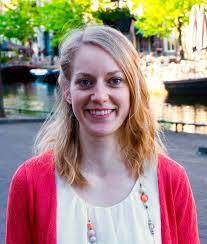
\includegraphics[width=\columnwidth,height=\paperheight,keepaspectratio]{../pictures/marthe.jpg}}
		\column{.7\textwidth}
		dr. A. Marthe Möller \\
		Assistant Professor Entertainment Communication
		\begin{itemize}
			\item Studying entertainment experiences in the digital space using:
			\begin{itemize}
				\item Computational methods (e.g., ACA of user comments)
				\item Experimental methods
			\end{itemize}
		\end{itemize}
		@marthemoller \textbar A.M.Moller@uva.nl \textbar \url{https://www.uva.nl/profiel/m/o/a.m.moller/a.m.moller.html} 
	\end{columns}
\end{frame}

\begin{frame}{Introducing\ldots \huge{Anne}} 
	\begin{columns}[] \column{.3\textwidth} \makebox[\columnwidth]{ 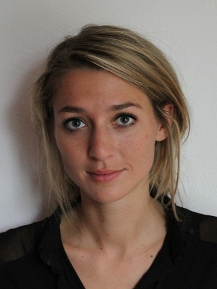
\includegraphics[width=\columnwidth,height=\paperheight,keepaspectratio]{../pictures/anne.jpg}} \column{.7\textwidth} dr. Anne Kroon \\ 
		Assistant Professor Corporate Communication
		\begin{itemize} 
			%\item Studied Journalism and Communication,  2006 - 2013
			%\item PhD candidate corporate communication at ASCoR (University of Amsterdam), 2014 - 2017
			\item Research focus on biased AI in recruitment, and media bias regarding minorities
			\item Text analysis using automated approaches, word embeddings
		\end{itemize} @annekroon \textbar a.c.kroon@uva.nl  \textbar \url{http://www.uva.nl/profiel/k/r/a.c.kroon/a.c.kroon.html} 
	\end{columns} 
\end{frame}


\begin{frame}{Introducing\ldots \huge{You}}
	{\huge{You}}
	\small{}
	\begin{columns}
		\column{.3\textwidth}
		\makebox[\columnwidth]{
			
\includegraphics[width=\columnwidth,height=\paperheight,keepaspectratio]{../pictures/mannetje.png}}
		\column{.7\textwidth}
		Your name?\\
		Your background?\\
		Your reason for taking this course?\\
		Do you have a dataset you are working on?
	\end{columns}
\end{frame}


\section{Introducing\ldots the course}


\begin{frame}{About CCS-2} 

What is CCS-2?
	\begin{itemize}
		\item Next step after CCS-1 %we assume you know the basics!
		\item How to use what you learned in CCS-1 for research?
		\begin{itemize}
			\item Learn computational techniques (e.g. data vectorization, machine learning)
			\item Learn how to use these techniques for research (e.g., content analysis)
		\end{itemize}
		\item By the end of the course, you'll be prepared to do computational research in the Research Project
	\end{itemize}
	
\end{frame}


\begin{frame}{About CCS-2}
	
	\begin{center}
		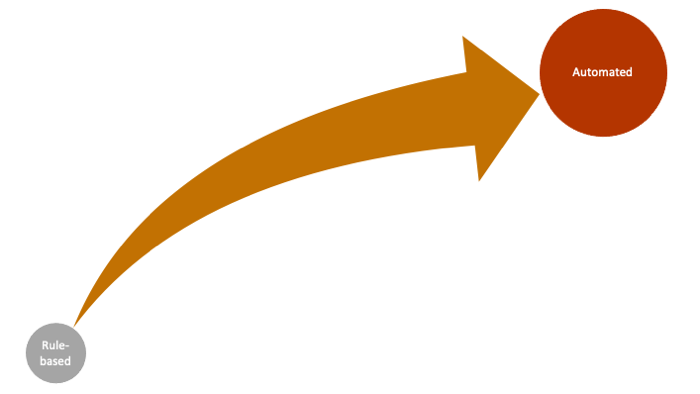
\includegraphics[width=\linewidth,height=\textheight,keepaspectratio]{../pictures/Roadmap.png} 
	\end{center}
	
\end{frame}


\begin{frame}{About CCS-2}
	
	\begin{center}
		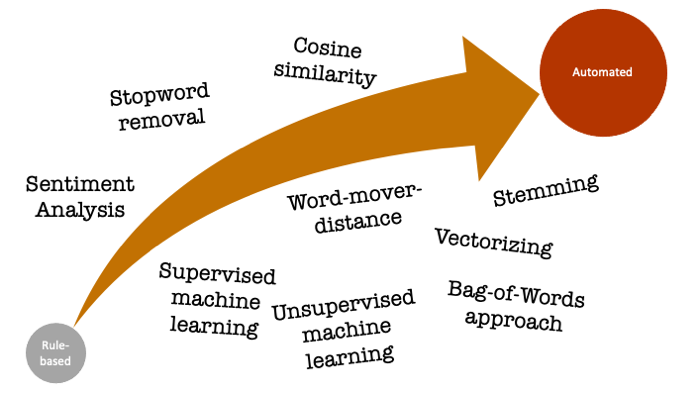
\includegraphics[width=\linewidth,height=\textheight,keepaspectratio]{../pictures/Roadmap_terms.png} 
	\end{center}
	
\end{frame}


\begin{frame}{About CCS-2} 

What will we do in this course?	
	\begin{itemize}
		\item We discuss techniques in the lectures
		\item We practice with techniques in the tutorials
		\item Graded assignments to master the techniques:
		\begin{itemize}
			\item Regular multiple choice questions (\(20\%\)) about readings that use the techniques we discuss
			\item Coding challenge (group assignment): Get more experienced with the techniques and build a recommender system
			\begin{itemize}
				\item Report (\(20\%\))
				\item Presentation (\(10\%\))
			\end{itemize}
			\item Take-home exam (\(50\%\)) at the end of the course so you can show off what you learned
		\end{itemize}
		\item We provide structure through the meetings and assignments, you do the (home-)work
	\end{itemize}
	
\end{frame}



\begin{frame}{About CCS-2} 
	
	How to stay informed and where to find all the materials? Regularly check:	
	\begin{itemize}
		\item The course Canvas page
		\item Your email
		\item The course Github page
	\end{itemize}

	In addition, make sure that you read the course manual so that you know all the ins and outs of this course!

\end{frame}


\begin{frame}{About CCS-2} 
	
	How to contact Anne and Marthe?	
	
	\textcolor{red}{We kunnen hier eventueel iets over zeggen: mogen ze mailen, zijn er spreekuren etc.?}
	
\end{frame}

\begin{frame}{Ready? Set? Go!} 
	
	Without further ado\dots
	
	\dots let's get started!
	
\end{frame}



\section{Text as Data}


\begin{frame}{Text as Data}
	
CCS-1: You learned how to...
	\begin{itemize}
	\item Work with Python, for example, you:
	\begin{itemize}
		\item Store text in json-files, csv-files etc.
		\item Work with texts in Python
	\end{itemize}
\end{itemize}
	
\end{frame}

\begin{frame}{Text as Data: \small{Learning from text directly}}
	
	Studying text can teach us a lot about human behavior: \\~
	
	What topics do people discuss on online cancer-related platforms? \\
	\begin{tiny}
		(\cite{sanders_different_2020}) \\
	\end{tiny}

	To what extent does content differ between online and print news? \\
	\begin{tiny}
	(\cite{burggraaff_through_2020}) \\
	\end{tiny}

	What topics do people discuss in their movie reviews? \\
	\begin{tiny}
	(\cite{schneider_what_2020}) \\
	\end{tiny}	

% Within communication science, text is often the subject of study
	
\end{frame}


\begin{frame}{Text as Data: \small{Analzing text as a means}}
	
	Studying text can give us information we can use to answer broader questions: \\~
	
	Analyze textual information about movies from IMDB to learn about the representation of women in movies \\
	\begin{tiny}
	(\cite{poma-murialdo_gender_2019}) \\
	\end{tiny}

	Automatically distinguish between reliable and unreliable online information about vaccines by investigating what characterizes reliable and unreliable texts \\
	\begin{tiny}
	(\cite{meppelink_reliable_2021}) \\
	\end{tiny}	
	
	% Within communication science, text is often the subject of study
	
\end{frame}


\begin{frame}{Text as Data: \small{Combining text analysis with other methods}}
	
	We can use data about text in combination with other methods: \\~
	
	Combining data about media content and survey data to investigate how media coverage affects citizens' trust in the EU \\
	\begin{tiny}
		(\cite{brosius_trust_2019}) \\
	\end{tiny}
	
	
	% Within communication science, text is often the subject of study
	
\end{frame}


\begin{frame}{Text as Data: NLP}
	
	"\textbf{Natural language processing (NLP)} refers to the branch of computer science — and more specifically, the branch of artificial intelligence or AI — concerned with giving computers the ability to understand text and spoken words in much the same way human beings can."  \\
	\tiny{(IBM, 2020)}
	
	
	% Within communication science, text is often the subject of study
	
\end{frame}





\section{Analyzing songtexts: NLP}

\begin{frame}[fragile]{Molly Malone}
	
\begin{lstlisting} 
MollyMalone = "In Dublin's fair city, where the girls are so pretty, I first set my eyes on sweet Molly Malone. As she wheeled her wheelbarrow, Through streets broad and narrow Crying, Cockles and mussels, alive, alive, oh! Alive, alive, oh, Alive, alive, oh, Crying, Cockles and mussels, alive, alive, oh."  
\end{lstlisting}
	

% Let's start with a simple example to get an understanding of what can be done when analyzing texts. For this example, we take part of the song text of the traditional song "Molly Malone"

\end{frame}


\begin{frame}[fragile]{Molly Malone}
	
\begin{lstlisting}
print(type(MollyMalone))
print(len(MollyMalone))
print(MollyMalone[0])
print(MollyMalone[-1:])
\end{lstlisting}
	
\begin{lstlistingoutput}
<class 'str'>
96
I
.
\end{lstlistingoutput}

% You can see that this datatype is a string that has 96 characters, the first one being I and the last one being a period.
\end{frame}



\begin{frame}[fragile]{NLTK}
	
%What if we wanted to learn more about this song. Say, we want to know what words are used most in this text.
%We can use the NLTK package to help us with this.
%For example, it can help us with tokenaization which we need to look at the individual words of the text.

NLTK: Natural Language Toolkit (www.nltk.org) \\

Tokenization: The process of breaking text (sentences, paragraphs, chapters, etc.) into smaller parts (individual sentences, words, etc.)


\end{frame}



\begin{frame}[fragile]{Tokenization}
	
\begin{lstlisting}		
MM_words = word_tokenize(MollyMalone)

print(MM_words)
\end{lstlisting}
	
\begin{lstlistingoutput}
['In', 'Dublin', "'s", 'fair', 'city', ',', 'where', 'the', 'girls', 'are', 'so', 'pretty', ',', 'I', 'first', 'set', 'my', 'eyes', 'on', 'sweet', 'Molly', 'Malone', '.', 'As', 'she', 'wheeled', 'her', 'wheelbarrow', ',', 'Through', 'streets', 'broad', 'and', 'narrow', 'Crying', ',', 'Cockles', 'and', 'mussels', ',', 'alive', ',', 'alive', ',', 'oh', '!', 'Alive', ',', 'alive', ',', 'oh', ',', 'Alive', ',', 'alive', ',', 'oh', ',', 'Crying', ',', 'Cockles', 'and', 'mussels', ',', 'alive', ',', 'alive', ',', 'oh', '.']
\end{lstlistingoutput}

% let's create a list with the 3 most common words in this sentence. We can see a few problems arise: first, one of the most common words is also a pretty meaningless word: 'and'. Let's clean up our data and remove the stopwords so that there are only meaningful words left!

\end{frame}


\begin{frame}[fragile]{Tokenization}
	
	\begin{lstlisting}		
		print(Counter(MM_words).most_common(3))
	\end{lstlisting}
	
	\begin{lstlistingoutput}
		[(',', 17), ('alive', 6), ('oh', 4)]
	\end{lstlistingoutput}
	
	% let's create a list with the 3 most common words in this sentence. We can see a few problems arise: first, one of the most common words is also a pretty meaningless word: 'oh'. Let's clean up our data and remove the stopwords so that there are only meaningful words left!
	
\end{frame}




\begin{frame}[fragile]{Removing Stopwords}
	
\begin{lstlisting}		
stopwords = ['in', 'the', 'and', 'a','I', 'she', 'her', 'are', 'so', 'on', 'me', 'my', 'mine', 'oh']
nostopwords = []

for word in MM_words:
	if word not in stopwords:
		nostopwords.append(word)


print(nostopwords)
\end{lstlisting}
	
\begin{lstlistingoutput}
['In', 'Dublin', "'s", 'fair', 'city', ',', 'where', 'girls', 'pretty', ',', 'first', 'set', 'eyes', 'sweet', 'Molly', 'Malone', '.', 'As', 'wheeled', 'wheelbarrow', ',', 'Through', 'streets', 'broad', 'narrow', 'Crying', ',', 'Cockles', 'mussels', ',', 'alive', ',', 'alive', ',', '!', 'Alive', ',', 'alive', ',', ',', 'Alive', ',', 'alive', ',', ',', 'Crying', ',', 'Cockles', 'mussels', ',', 'alive', ',', 'alive', ',', '.'] 
\end{lstlistingoutput}

%The easiest way to do this is to create list with stopwords and then loop over our text and filter out the words in our text that are also in our stopwords-list.

%Of course, it is a bit of a hassle if we need to make such a list ourselves all the time. But there are files available online that contain stopwords and we can also just load those files and use them! --> The NLTK package has such a list.
\end{frame}


\begin{frame}[fragile]{Removing Stopwords}
	
	\begin{lstlisting}		
print(Counter(nostopwords).most_common(3))
	\end{lstlisting}
	
	\begin{lstlistingoutput}

[(',', 17), ('alive', 6), ('.', 2)]
	\end{lstlistingoutput}
	
	%The easiest way to do this is to create list with stopwords and then loop over our text and filter out the words in our text that are also in our stopwords-list.
	
	%Of course, it is a bit of a hassle if we need to make such a list ourselves all the time. But there are files available online that contain stopwords and we can also just load those files and use them! --> The NLTK package has such a list.
\end{frame}



\begin{frame}[fragile]{Removing Stopwords}
	
	\begin{lstlisting}		
		from nltk.corpus import stopwords
		
		print(len(stop_words))
	\end{lstlisting}
	
	\begin{lstlistingoutput}
		179
	\end{lstlistingoutput}

\end{frame}



\begin{frame}[fragile]{Removing Stopwords}
	
	\begin{lstlisting}		
nostopwords = []

for word in MM_words:
	if word not in stop_words:
		nostopwords.append(word)


print(nostopwords)
	\end{lstlisting}
	
	\begin{lstlistingoutput}
['In', 'Dublin', "'s", 'fair', 'city', ',', 'girls', 'pretty', ',', 'I', 'first', 'set', 'eyes', 'sweet', 'Molly', 'Malone', '.', 'As', 'wheeled', 'wheelbarrow', ',', 'Through', 'streets', 'broad', 'narrow', 'Crying', ',', 'Cockles', 'mussels', ',', 'alive', ',', 'alive', ',', 'oh', '!', 'Alive', ',', 'alive', ',', 'oh', ',', 'Alive', ',', 'alive', ',', 'oh', ',', 'Crying', ',', 'Cockles', 'mussels', ',', 'alive', ',', 'alive', ',', 'oh', '.']
	\end{lstlistingoutput}
	
\end{frame}



\begin{frame}[fragile]{Molly Malone}
	
\begin{lstlisting}
print(Counter(nostopwords).most_common(3))
	\end{lstlisting}
	
\begin{lstlistingoutput}
[(',', 17), ('alive', 6), ('oh', 4)]
\end{lstlistingoutput}
	
 %As you can see, in the ready-made stopword list, 'oh' was not included in a stopwords and it is therefore still there. In this case, we can add this as a stopword to the NLTK list to customize it for our research.
 
 %But still we see that the most commonly used "word" is the comma. But this is not a word!
	
	% In a similar way that we removed the stopwords, let's remove punctuation from the text!
	
\end{frame}



\begin{frame}[fragile]{Molly Malone}
	
	\begin{lstlisting}
import string
punct = list(string.punctuation)
print(punct[:5])
	\end{lstlisting}
	
	\begin{lstlistingoutput}
		['!', '"', '#', '$', '%']
	\end{lstlistingoutput}
	
	% Again, we can use a ready made collection of punctuation marks for this. 

	
\end{frame}



\begin{frame}[fragile]{Molly Malone}
	
	\begin{lstlisting}
nostopnopunct = []

for word in nostopwords:
if word not in punct:
nostopnopunct.append(word)


print(nostopnopunct)
	\end{lstlisting}
	
	\begin{lstlistingoutput}
['In', 'Dublin', "'s", 'fair', 'city', 'where', 'girls', 'pretty', 'first', 'set', 'eyes', 'sweet', 'Molly', 'Malone', 'As', 'wheeled', 'wheelbarrow', 'Through', 'streets', 'broad', 'narrow', 'Crying', 'Cockles', 'mussels', 'alive', 'alive', 'Alive', 'alive', 'Alive', 'alive', 'Crying', 'Cockles', 'mussels', 'alive', 'alive']
	\end{lstlistingoutput}
	

	%Now you can see that the computer removed all the comma's, periods, and exclamation marks.
	
\end{frame}





\begin{frame}[fragile]{Molly Malone}
	
\begin{lstlisting}
print(Counter(nostopnopunct).most_common(3))
\end{lstlisting}
	
\begin{lstlistingoutput}
[('alive', 6), ('Crying', 2), ('Cockles', 2)]
\end{lstlistingoutput}
	

%However, one thing is still not quite correct. It says that the most common word is 'alive' and that this word occurs 6 times. But if we cound ourselves, we see that it is in fact used 8 times. However, sometimes it has a capital letter and sometimes it doesn't. Let's remove the capital letters.
\end{frame}



\begin{frame}[fragile]{Molly Malone}
\begin{lstlisting}
lower = []

for word in nostopnopunct:
lower.append(word.lower())

print(lower)
\end{lstlisting}

\begin{lstlistingoutput}
['in', 'dublin', "'s", 'fair', 'city', 'where', 'girls', 'pretty', 'first', 'set', 'eyes', 'sweet', 'molly', 'malone', 'as', 'wheeled', 'wheelbarrow', 'through', 'streets', 'broad', 'narrow', 'crying', 'cockles', 'mussels', 'alive', 'alive', 'alive', 'alive', 'alive', 'alive', 'crying', 'cockles', 'mussels', 'alive', 'alive']
\end{lstlistingoutput}

%The lower-function allows us to do this.
\end{frame}


\begin{frame}[fragile]{Molly Malone}
\begin{lstlisting}
print(Counter(lower).most_common(3))
\end{lstlisting}

\begin{lstlistingoutput}
[('alive,', 8), ('crying', 2), ('cockles', 2)]
\end{lstlistingoutput}

%Now, we see that the computer correctly counted all 8 times the word 'alive' was used.

\end{frame}


\section{Analyzing songtexts: RegEx}


\begin{frame}{Note}
	
	Hier moet ook nog iets over search vs findall etc.

\end{frame}

\begin{frame}[fragile]{RegEx}
	
	"A \textit{regular expression} or \textit{regex} is a powerful language to locate strings that conform to a given pattern. [...] Specifically, regular expressions are a sequence of characters that we can use to design a pattern and then use this pattern to \textit{find} strings (identify or extract) and also \textit{replace} those strings by new ones." \\
	\begin{tiny}
		\cite{van_atteveldt_computational_2022} 
	\end{tiny}
	

\end{frame}


\begin{frame}[fragile]{RegEx}

\begin{lstlisting}
for word in MollyMalone_words:
	if re.search("[Aa]live", word):
		print(word)
\end{lstlisting}
	
\begin{lstlistingoutput}
		alive
		alive
		Alive
		alive
		Alive
		alive
		alive
		alive
\end{lstlistingoutput}
	
	%For example, instead of first making everything in Molly Malone's lyrics lowercase, we could also use regular expressions to find the word "alive" (with and without capital).
	
\end{frame}



\begin{frame}[fragile]{RegEx}

\lstinline{m[oa]lly} matches molly, but also mally \\
\lstinline{m.lly} matches molly, but also mally, or melly, or milly...

	
	%RegEx has some wildcards. 
	
\end{frame}


\begin{frame}[fragile]{Quantifiers}
	
\lstinline{mol+y} matches moly, molly, mollly, molllly...  \\
\lstinline{[mM]ol+y} matches moly, molly, and mollly, but also Moly, Molly, Mollly, Molllly... 
	
	
	%You can also specify how often you want a character to occur.

	
\end{frame}


\begin{frame}[fragile]{Quantifiers}
	
	<b>Molly Malone</b> \\
	\lstinline{<.*>} is greedy and will select everything   \\
	\lstinline{<.*?>} is non-greedy and will match <b> and </b>

	
	
	%Note that by default, quantifiers are greedy, meaning that they will match as many characters as possible.
	
\end{frame}


\begin{frame}[fragile]{Groups}
	
	\lstinline{That was (not)? the end of sweet Molly Malone} \\ 
	will select both:   \\
	That was the end of sweet Molly Malone and That was not the end of sweet Molly Malone
		
	%You can use brackets to create groups.
	
\end{frame}


\begin{frame}[fragile]{Character classes}
	
	
	The Dublin Millennium Commission proclaimed 13 June to be "Molly Malone Day"
	\lstinline{[1-9]+.[A-Z][a-z]+} \\ 
	will select 13 June

	
	%With character classes, you can specify a number of different characters that you want to match. You can use - to indicate a range.
	
% more examples of regular expressions
%practice using: https://regexr.com/6dhpi --> find all the dates mentioned in the text

\end{frame}


\begin{frame}{Note}
	
	En ook iets met stemming en lemming --> dus dan combineer je NLTK met Regex; wheeled wheelbarrow

\end{frame}


\begin{frame}{note}
	
	En dan eindigen met: terug naar onderzoek, wat kun je hier nu precies mee?
	En dan noem je de Twitter-artikelen als voorbeeld, zodat er weer terugkoppeling is van pietje-precieze code dingen naar onderzoek
	
	+ schietgebedje dat het niet allemaal veeeeel te veel is :) 
	
\end{frame}


\end{document}